\documentclass[tikz]{standalone}
\usepackage[T1]{fontenc}
\usepackage{mathpazo} % Palatino font
\usepackage{pgfplots}
\pgfplotsset{compat=1.18}
 \usetikzlibrary{arrows.meta}

\begin{document}
% Preamble:
% \usepackage{tikz}
% \usetikzlibrary{arrows.meta}

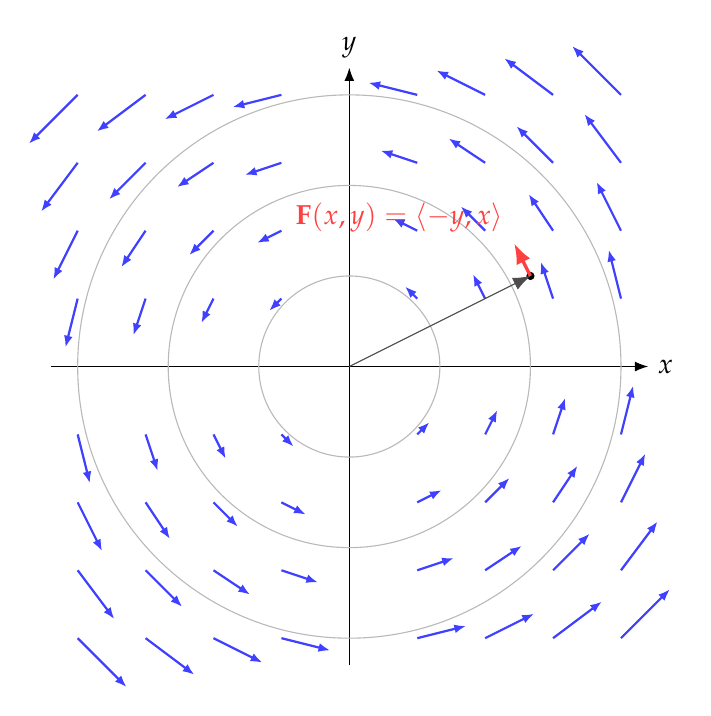
\begin{tikzpicture}[scale=1.15,>=Latex]
	
	% --- Axes
	\draw[->] (-3.3,0) -- (3.3,0) node[right] {$x$};
	\draw[->] (0,-3.3) -- (0,3.3) node[above] {$y$};
	
	% --- Reference circles (streamlines): x^2+y^2 = const
	\draw[gray!55] (0,0) circle (1);
	\draw[gray!55] (0,0) circle (2);
	\draw[gray!55] (0,0) circle (3);
	
	% --- Vector field F(x,y)=<-y,x> (counterclockwise rotation)
	% Use a small grid; arrows get longer as r increases.
	\foreach \x in {-3,-2.25,-1.5,-0.75,0.75,1.5,2.25,3}{
		\foreach \y in {-3,-2.25,-1.5,-0.75,0.75,1.5,2.25,3}{
			% Skip near the origin to avoid tiny/degenerate arrows
			\pgfmathsetmacro{\r}{sqrt((\x)^2+(\y)^2)}
			\ifdim \r pt > 0.55pt
			% Vector is (-y,x); scale factor controls arrow length in the picture.
			\pgfmathsetmacro{\sx}{0.18}
			\pgfmathsetmacro{\vx}{-\sx*(\y)}
			\pgfmathsetmacro{\vy}{ \sx*(\x)}
			\draw[blue!75, -{Latex[length=1.5mm]}, thick] (\x,\y) -- ++(\vx,\vy);
			\fi
		}
	}
	
%	% --- Mark a sample point and show orthogonality / tangency visually
	\coordinate (P) at (2,1);
	\draw[black, fill=black] (P) circle (1.1pt) node[above right] {};
	
	% Radial vector <x,y> from origin to P (points outward)
	\draw[black!70, -{Latex[length=2.2mm]}] (0,0) -- (P) node[midway, below right] {};
	
	% Field vector at P is <-y,x> = <-1,2> (tangent, CCW)
	\draw[red!75, very thick, -{Latex[length=2.6mm]}] (P) -- ++(-0.18*1,0.18*2)
	node[above left] {$\mathbf F(x,y)=\langle -y,x\rangle$};
	
%	% Right-angle marker to emphasize perpendicularity at P
%	\begin{scope}[shift={(P)}]
%		% small right angle box between radial direction and field direction
%		\pgfmathsetmacro{\a}{atan2(1,2)} % angle of radial vector from origin to (2,1)
%		\draw[black!70] (0,0) --
%		++({0.22*cos(\a)},{0.22*sin(\a)}) --
%		++({0.22*cos(\a+90)},{0.22*sin(\a+90)}) --
%		++({-0.22*cos(\a)},{-0.22*sin(\a)});
%	\end{scope}
	
	% --- Caption
%	\node[align=left] at (0,-3.85) {\small
%		$\mathbf F(x,y)=\langle -y,x\rangle$ is tangent to circles $x^2+y^2=\text{const}$ and rotates CCW;\\[-1pt]
%		$\|\mathbf F(x,y)\|=\sqrt{x^2+y^2}$ grows linearly with distance from the origin.};
	
\end{tikzpicture}
\end{document}
